\documentclass[conference]{IEEEtran}
\IEEEoverridecommandlockouts
% The preceding line is only needed to identify funding in the first footnote. If that is unneeded, please comment it out.
\usepackage{cite}
\usepackage{amsmath,amssymb,amsfonts}
\usepackage{algorithmic}
\usepackage{graphicx}
\usepackage{url}
\usepackage[utf8]{inputenc}
\usepackage{textcomp}


\usepackage[english,ngerman,brazilian]{babel}
\def\BibTeX{{\rm B\kern-.05em{\sc i\kern-.025em b}\kern-.08em
    T\kern-.1667em\lower.7ex\hbox{E}\kern-.125emX}}
\begin{document}

\title{Projeto Demonstrativo 3 - Múltiplas Vistas}

\author{\IEEEauthorblockN{Frederico Guth (18/0081641)}
\IEEEauthorblockA{\textit{Tópicos em Sistemas de Computação, ,} \\
\textit{Turma TC - Visão Computacional (PPGI)}\\
\textit{Universidade de Brasília}\\
Brasília, Brasil\\
fredguth@fredguth.com}
}

\maketitle

\begin{abstract}
Quando duas câmeras capturam a mesma cena, com centros de projeção não coincidentes, cada par de imagem capturado por essas câmeras representa duas perspectivas diferentes de uma mesma cena estática. Neste projeto usaremos geometria estéreo para reconstruir a cena 3D, criando um mapa de profundidade da mesma.
\end{abstract}

\begin{IEEEkeywords}
câmeras, calibração estéreo, mapa de profundidade
\end{IEEEkeywords}

\section{Introdução}
Quando duas câmeras capturam a mesma cena, com centros de projeção não coincidentes, cada par de imagem capturado por essas câmeras representa duas perspectivas diferentes de uma mesma cena estática. A partir dessas perspectivas e da correspondência de pontos entre elas é possível reconstruir a cena 3D, posicionando as câmeras e demais objetos através de uma triangulação.

O mapa de profundidade, armazena as profundidades estimadas para cada ponto de uma imagem 2D, representando a estrutura 3D da cena. A Figura {xyz} mostra o mapa de profundidade computado por uma triangulação dos pontos correspondentes e não ocluídos das imagens (a) e (b). As áreas mais claras representam as profundidades mais próximas da câmera, equanto as áreas escuras, as mais distantes.

\subsection{Objetivos}
Este projeto tem como objetivo principal a exploração e desenvolvimento de algoritmos para extração de mapas de profundidade a partir de pares estéreo de imagens.

Mais especificamente deseja-se:
\begin{enumerate}
\item estimar o mapa de profundidade de imagens estéreos já pre-processadas onde se sabe que as linhas epipolares são perfeitamente horizontais;
\item gerar mapas de profundidade a partir de um par de imagens da mesma cena, usando pares de imagens capturadas no projeto, não pré-processadas;
\item medir um objeto através de sua imagem e comparar com suas dimensões reais;
\item analisar os resultados obtidos.
\end{enumerate}
\section{Revisão Teórica}

O cálculo da profundidade requer o conhecimento da disparidade entre pontos correspondentes nas perspectivas, ou seja, a distância entre as projeções 2D de um mesmo ponto no espaço 3D de cada câmera.

A busca por pontos correspondentes pode ser realizada levando-se em consideração a restrição epipolar, que restringe a busca de um dado ponto x da primeira imagem a uma linha epipolar na segunda imagem.

Para facilitar, ainda é possível retificar as imagens, que transforma cada plano das imagens de forma que as linhas epipolares em paralelas horizontais, perimtindo que buscas mais simples, linha a linha da imagem.

Na busca por pontos correspondentes, empregando um par de imagens retificadas, a medida de disparidade \(d\), que é a diferança em pixels entre os pontos correspontens nas imagens de cada uma das câmeras, pode ser usada para obter o valor de profundidade \(z\) pela relação definida em {livro} como

\(z = b f /d \)

em que \(b\) é a distância entre os centros de projeção das câmeras (baseline) e f é a distância focal. 
\section{Metodologia}\label{metodologia}
O modelo da câmera e seus parâmetros foram descritos na seção de Revisão Teórica. Nesta seção, descreve-se como estimá-los experimentalmente.

\subsection{Materiais}
Foram utilizados:
\begin{itemize}

\item fita adesiva
\item padrões de calibração xadrez impressos em papel A4
\item uma trena
\item uma régua
\item computador MacBook Pro (Retina, 13-inch, Early 2015), Processador Intel Core i5 2,7 GHz, 8GB de RAM
\item Python 3.6.3 :: Anaconda custom (64-bit)
\item OpenCV 3.4.0
\item programas em python especialmente desenvolvidos para o projeto. Todos estão disponíveis no repositório: \url{git@github.com:fredguth/unb-cv-3183.git}\label{repo}
\end{itemize}



\section{Resultados}
Nesta seção apresentamos, para cada etapa da \ref{metodologia}, os resultados obtidos. Todos os dados podem ser acessados no repositório do projeto (\ref{repo}).

\subsection{Mapas de profundidade de imagens estéreo já pré-processadas}


\begin{figure}[ht!]\label{aloeDisp}
\begin{center}
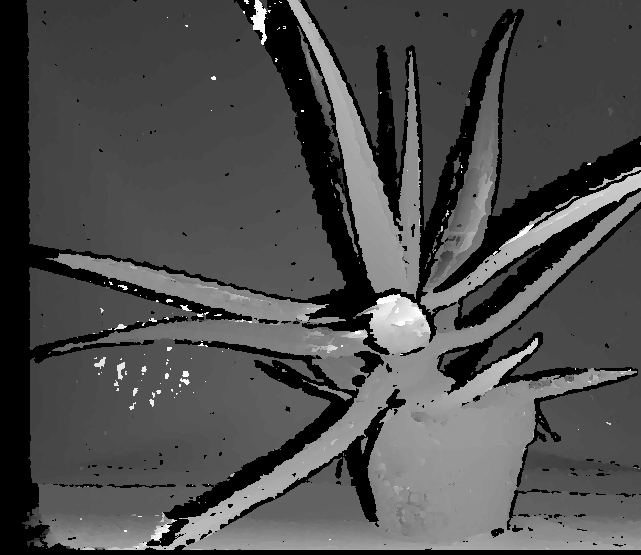
\includegraphics[width= .85\columnwidth]{aloeDisp.png}
\caption{Mapa de disparidade da imagem Aloe}
\end{center}
\end{figure}

\begin{figure}[ht!]\label{aloeDepth}
\begin{center}
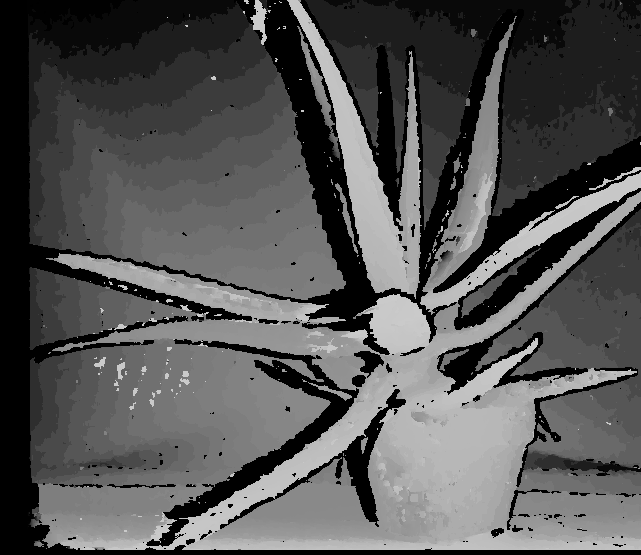
\includegraphics[width= .85\columnwidth]{aloeDepth.png}
\caption{Mapa de profundidade da imagem Aloe}
\end{center}
\end{figure}

\begin{figure}[ht!]\label{babyDisp}
\begin{center}
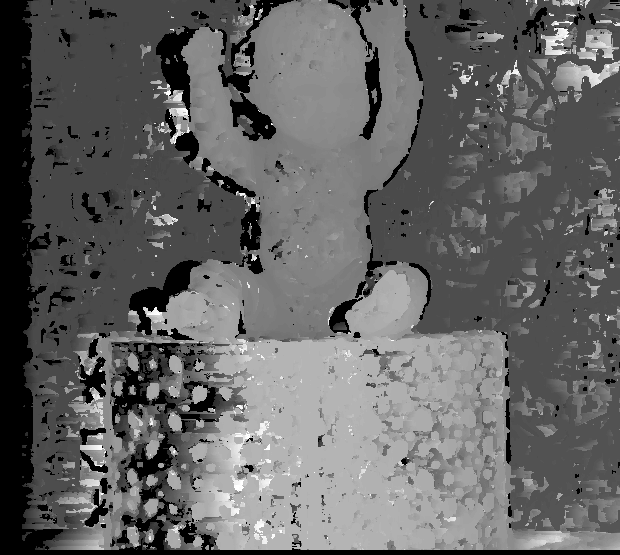
\includegraphics[width= .85\columnwidth]{babyDisp.png}
\caption{Mapa de disparidade da imagem Baby}
\end{center}
\end{figure}

\begin{figure}[ht!]\label{babyDepth}
\begin{center}
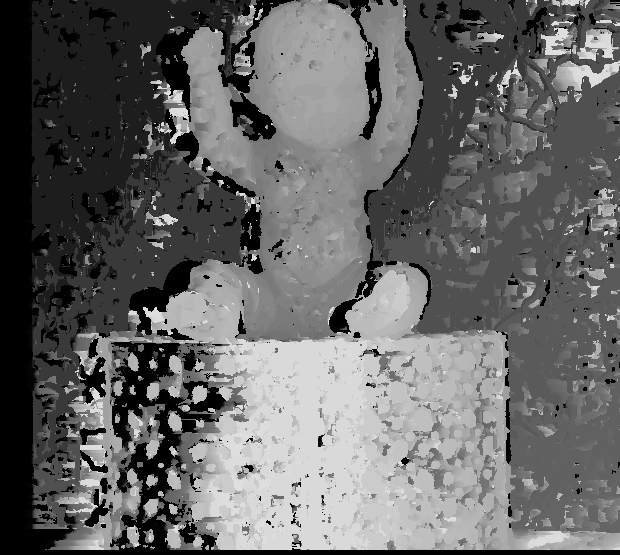
\includegraphics[width= .85\columnwidth]{babyDepth.png}
\caption{Mapa de profundidade da imagem Baby}
\end{center}
\end{figure}

\subsection{Mapa de profundidade de imagens não processadas}

\begin{figure}[ht!]\label{retificacao}
\begin{center}
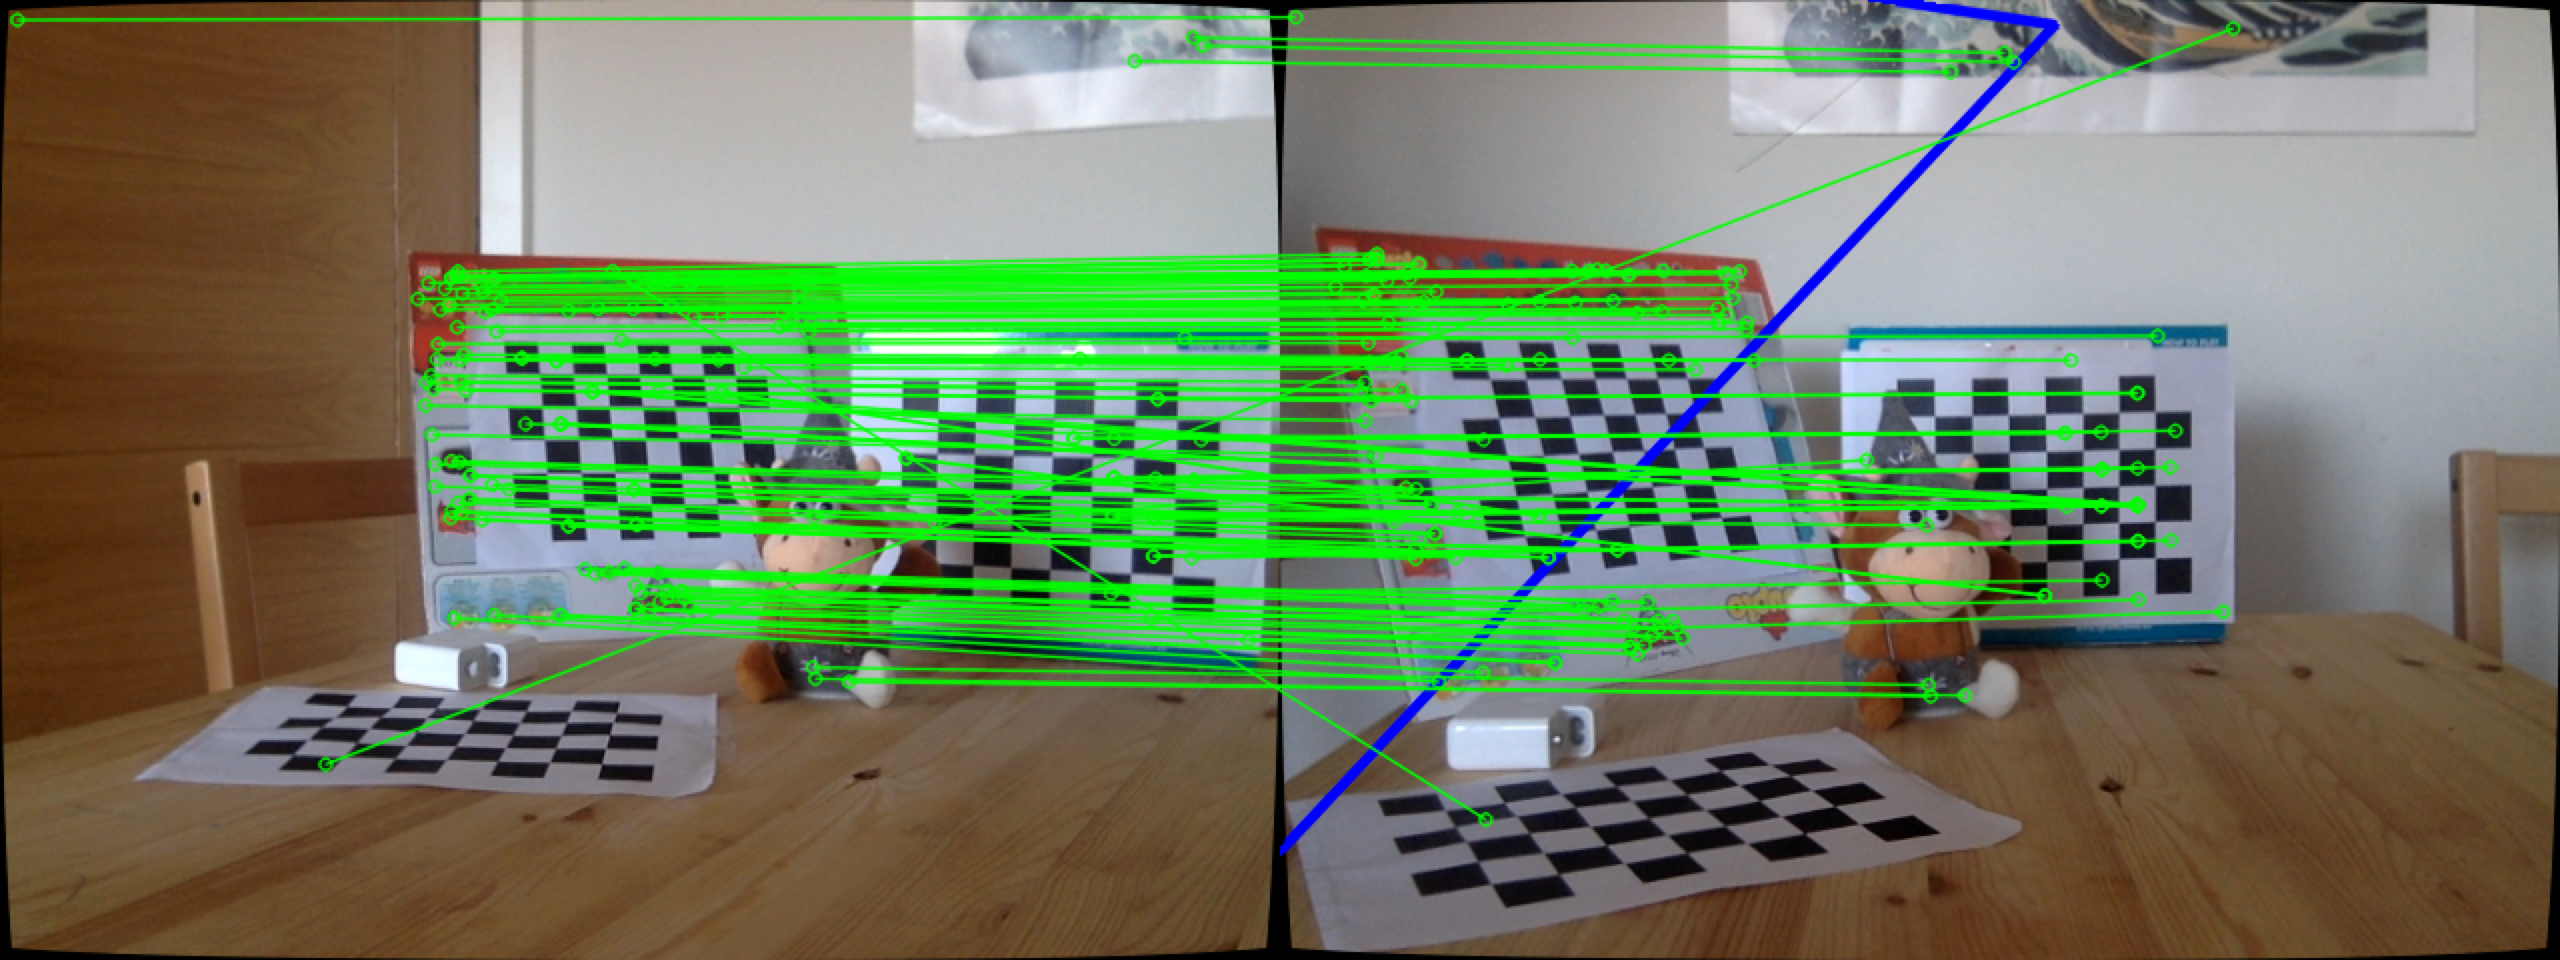
\includegraphics[width= .85\columnwidth]{retificacao.png}
\caption{Processo de retificaçao, encontrando correspondencias}
\end{center}
\end{figure}

\section{Discussão e Conclusões}

% \begin{figure}[htbp]
% \centerline{
\includegraphics{fig.jpg}}
% \caption{Example of a figure caption.}
% \label{fig}
% \end{figure}

\selectlanguage{brazilian}
\bibliographystyle{IEEEtran}
\bibliography{references}

\end{document}
